\documentclass[12pt, a4paper]{exam}
\usepackage{graphicx}
\usepackage[left=0.8in, top=0.7in, total={6.2in,8in}]{geometry}
\usepackage[normalem]{ulem}
\renewcommand\ULthickness{1.0pt}   %%---> For changing thickness of underline
\setlength\ULdepth{1.3ex}%\maxdimen ---> For changing depth of underline
\usepackage[cmex10]{amsmath}

\begin{document}
	%\thispagestyle{empty}
	\noindent
	\begin{minipage}[l]{0.1\textwidth}
		\noindent
		
\includegraphics[width=1.6\textwidth]{figs/logo.png}
	\end{minipage}
\hfill
\begin{minipage}[c]{0.8\textwidth}
	\begin{center}
		\large	Indian Institute of Technology Hyderabad \par
		%\large	Department of Electrical Engineering	\par
		\large	Future Wireless Communitcation \par
	\large \textbf{Entrace Exam}%	\par
%\small	Date: Feb 25, 2020}
	\end{center}
\end{minipage}
\par
\vspace{0.2in}
\noindent
\uline{Duration: 30 min \hfill Date: Jun 28, 2023}%	\hfill Max mark: 10}
\par 
\vspace{0.15in}
\noindent
\centering
%{\small \bfseries 	Attempt any five questions }

\begin{questions}
	\pointsdroppedatright
%	\question
%	In the given figure, $ \angle{AOB} = 90^{\circ}$ and $\angle{ABC } = 30^{\circ}$ , then $\angle{CAO}$ is equal to %\textbf{\droppoints}
%
%	\begin{figure}[h!]
%	\centering
%	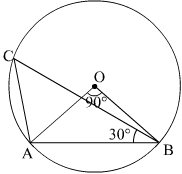
\includegraphics[width=0.27\textwidth]{figs/Q1.png}
%	\end{figure}

	\question
	What is the value of  \angle ABC ?
	\begin{figure}[h!]
	\centering
	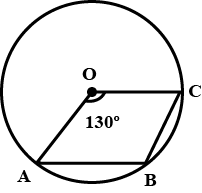
\includegraphics[width=0.4\textwidth]{figs/2.png}
	\end{figure}
	%answer = 120/17

	\question
 A train can travel 50\% faster than a car. Both start from point A at the same time and reach point B 75 kms away from A at the same time. On the way, however, the train lost about 12.5 minutes while stopping at the stations. The speed of the car is ?
	%answer = 13
	%https://www.math10.com/problems/arithmetic-progression-problems/difficult/
	
\end{questions}
\vspace{0.75in}
{\large \bfseries Best wishes}
\end{document}
